%%%%%%%%%%%%%% 03/03/2020 %%%%%%%%%%%%%%%% 
\subsection*{\textbf{03/03/2020}}
\subsubsection{Days Aim}
\begin{itemize}
    \item Estimate the uncertainty on $\sigma (Z \rightarrow ee)$ and $\sigma (Z \rightarrow \mu\mu)$
\end{itemize}
\subsubsection{Day Summary}
\begin{itemize}
    \item Cut on pT
    \subitem $Z \rightarrow ee$ = $26 GeV < p_T$
    \subitem $Z \rightarrow \mu\mu$ = $28 GeV < p_T$

    \item Cut on ptcone30
    \subitem $Z \rightarrow ee$ = $ ptcone < 5.8 GeV$
    \subitem $Z \rightarrow \mu\mu$ = $ ptcone < 6.5 GeV$

    \item Cut on etcone20
    \subitem $Z \rightarrow ee$ = $ -2 GeV < etcone < 6 GeV$
    \subitem $Z \rightarrow \mu\mu$ = $ -1.6 GeV < etcone < 5.25 GeV$

    \item Cut on invariant mass
    \subitem $Z \rightarrow ee$ = $65 GeV < m_{ll} < 150 GeV$
    \subitem $Z \rightarrow \mu\mu$ = $65 GeV < m_{\mu\mu} < 150 GeV$
    
    \item Systematic uncertainty on $\sigma (Z \rightarrow ee)$ due to $p_T$ variations to be: 
    \subitem
    
    \item Systematic uncertainty on $\sigma (Z \rightarrow ee)$ due to $m_{ee}$ variations to be: 
    \subitem
    
    \item Systematic uncertainty on $\sigma (Z \rightarrow \mu\mu)$ due to $p_T$ variations to be: 
    \subitem
    
    \item Systematic uncertainty on $\sigma (Z \rightarrow \mu\mu)$ due to $m_{\mu\mu}$ variations to be: 
    \subitem
\end{itemize}
%%%%%%%%%%%%% 09:48 %%%%%%%%%%%%%
\subsubsection*{09:48 - Lead BG - Plotting the PT for ee (with full cuts)}
Plotting the transverse momentum for $Z \rightarrow ee$ as a stack plot (fast).
\\
Cuts used in Fig.\ref{fig:09-48_03-03-21}:
\begin{lstlisting}
basic_cut = "(lep_charge[0] != lep_charge[1]) && (lep_type[0] == 11 && lep_type[1] == 11) && lep_n==2"

inv_mass_cut = "(inv_mass_Zll > 70e3) && (inv_mass_Zll < 150e3)"

etcone_cut = "(lep_etcone20[0] > -2e3 && lep_etcone20[1] > -2e3)" + "&& (lep_etcone20[0] < 6e3 && lep_etcone20[1] < 6e3)"

ptcone_cut = "(lep_ptcone30[0] < 5.8e3) && (lep_ptcone30[1] < 5.8e3)"

lepCut = "(" + basic_cut + "&&" + inv_mass_cut + "&&" + etcone_cut + "&&" + ptcone_cut + ")"

t.SetAlias("inv_mass_Zll","sqrt(2*lep_pt[0]*lep_pt[1]*(cosh(lep_eta[0]-lep_eta[1])-cos(lep_phi[0]-lep_phi[1])))")

t.Draw("lep_pt[1] >> h_lep_pt_total(100, 0,100e3)", weighting + "*" + lepCut)
\end{lstlisting}

\begin{figure}[h!]
    \centering
    \begin{minipage}{0.5\textwidth}
        \centering
        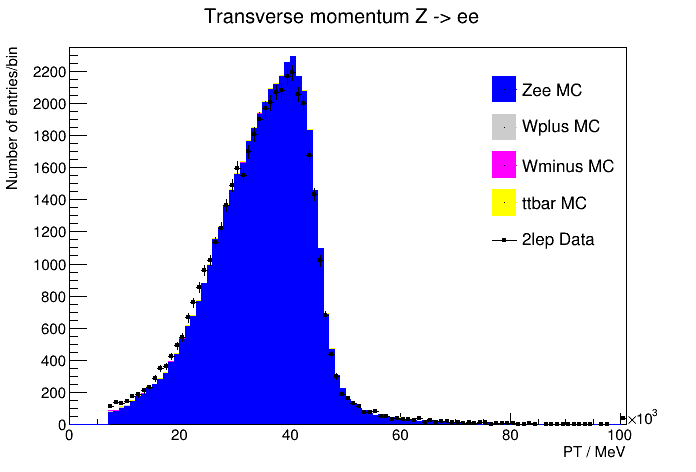
\includegraphics[width=\linewidth]{plots/03-03-2021/09-48_03-03-21.png}
        (A)
    \end{minipage}\hfill
    \begin{minipage}{0.5\textwidth}
        \centering
        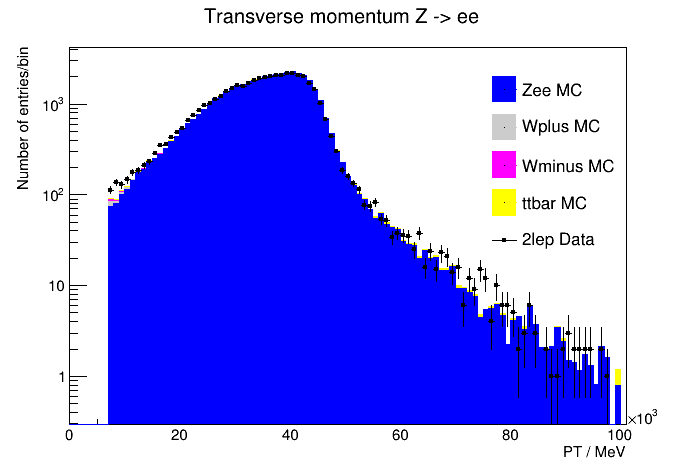
\includegraphics[width=\linewidth]{plots/03-03-2021/09-49_03-03-21.png}
        (B)
    \end{minipage}
    \caption{(A) Transverse momentum of ee pair for a single lepton with ATLAS, Signal, and background MC data. (B) Transverse momentum of ee pair with ATLAS, Signal, and background MC data - log-y plot.  Cuts: electron pair with opposite charge, $70 GeV < m_{ee} < 150 GeV$, $36 GeV < p_T$, $ ptcone < 5.8 GeV$, $ -2 GeV < etcone < 6 GeV$.}
    \label{fig:09-48_03-03-21}
\end{figure}
Cut to be made for $Z \rightarrow ee$:
\begin{align}
    p_T > 26 GeV    
\end{align}


\subsubsection*{10:30 - Plotting $m_{ll}$ for ee (with full cuts)}
Plotting the invariant mass for $Z \rightarrow ee$ as a stack plot (fast).
\\
Cuts used in Fig.\ref{fig:10-30_03-03-21}:
\begin{lstlisting}
basic_cut = "(lep_charge[0] != lep_charge[1]) && (lep_type[0] == 11 && lep_type[1] == 11) && lep_n==2"

etcone_cut = "(lep_etcone20[0] > -2e3 && lep_etcone20[1] > -2e3)" + "&& (lep_etcone20[0] < 6e3 && lep_etcone20[1] < 6e3)"

ptcone_cut = "(lep_ptcone30[0] < 5.8e3) && (lep_ptcone30[1] < 5.8e3)"

pt_cut = "(lep_pt[0] > 26e3) && (lep_pt[1] > 26e3)"
    
lepCut = "(" + basic_cut + "&&" + etcone_cut + "&&" + ptcone_cut + "&&" + pt_cut + ")"
    
t.SetAlias("inv_mass_Zll","sqrt(2*lep_pt[0]*lep_pt[1]*(cosh(lep_eta[0]-lep_eta[1])-cos(lep_phi[0]-lep_phi[1])))")
  
t.Draw("inv_mass_Zll >> h_inv_mass(100,0,150e3)", weighting + "*" + lepCut)
\end{lstlisting}
\begin{figure}[h!]
    \centering
    \begin{minipage}{0.5\textwidth}
        \centering
        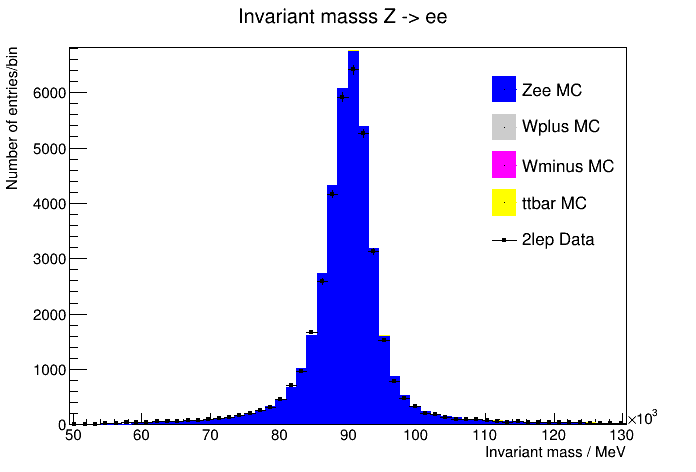
\includegraphics[width=\linewidth]{plots/03-03-2021/10-30_03-03-21.png}
        (A)
    \end{minipage}\hfill
    \begin{minipage}{0.5\textwidth}
        \centering
        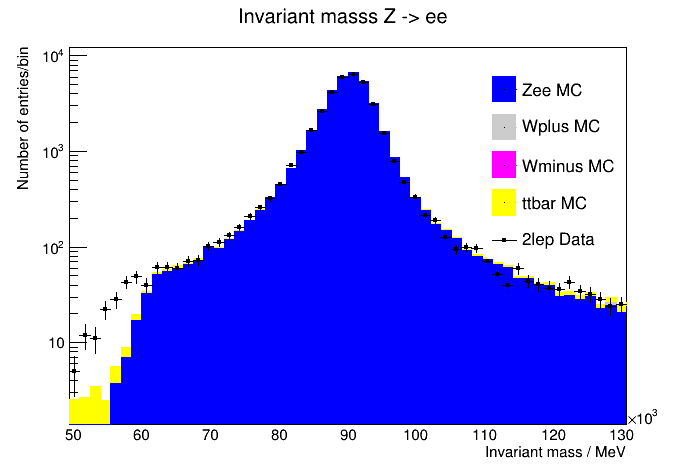
\includegraphics[width=\linewidth]{plots/03-03-2021/10-31_03-03-21.png}
        (B)
    \end{minipage}
    \caption{(A) Invariant mass of ee pair with ATLAS, Signal, and background MC data. (B) Transverse momentum of mumu pair with ATLAS, Signal, and background MC data - log-y plot.  Cuts: electron pair with opposite charge, $36 GeV < p_T$, $ ptcone < 5.8 GeV$, $ -2 GeV < etcone < 6 GeV$, $p_T > 26 GeV $.}
    \label{fig:10-30_03-03-21}
\end{figure}

Cuts on Invariant mass for $Z \rightarrow ee$
\begin{align}
    65 GeV < m_{ee} < 150 GeV
\end{align}

%%%%%%%%%%%%% 11:00 %%%%%%%%%%%%%

\begin{figure}[h!]
    \centering
	\includegraphics[width=0.85\linewidth]{plots/03-03-2021/}
    \caption{Cross sections of $\sigma (Z \rightarrow ee)$ as the cut on the cut on the invariant mass changes}
    \label{fig:13:00_03-03-21}
\end{figure}
The systematic uncertainty as the invariant mass cut change:
\begin{align}
    ...
\end{align}


